\chapter{Objetivos}\label{cap.objetivos}
\hspace{1cm} Una vez introducidas las motivaciones que han llevado a hacer este Trabajo Fin de Grado y expuesto el contexto, en este capítulo se van a exponer los diferentes problemas concretos que se abordarán, los requisitos para las soluciones desarrolladas y por último la metodología y el plan de trabajo que se ha seguido. 


\section{Problemas a abordar}
\hspace{1cm} El objetivo principal de este trabajo es la creación de un sistema  que permita el funcionamiento de un dron completamente autónomo que despegue de forma controlada, siga una ruta previamente establecida y aterrice tambien de forma controlada. Para la parte de enrutamiento el drone ha de conocer en todo momento su posición en
el entorno mediante técnicas de visión por computador basadas en marcadores visuales artificiales, mientras que para el despegue y aterrizaje controlados debe reconocer las balizas por visión cuya posición es desconocida. 

\hspace{1cm} Este objetivo se ha desglosado en varios subobjetivos para abordarlo por partes:

\begin{enumerate}
	\item{\textbf{Adaptación e integración del módulo de autolocalización visual:} Este módulo proporciona la posición absoluta del drone en el mundo basándose en la detección de balizas visuales y cálculos geométricos. Existía una versión previa debida al TFM de Alberto y al PFC de Manuel, pero nadie la había integrado dentro de un automata de estados finito, para ello hemos ajustado el componente y lo hemos introducido por pasos para finalmente conseguir su correcto funcionamiento.}
	\item{\textbf{Adaptación e integración del módulo de aterrizaje visual:} Este módulo se encarga de controlar al drone para que se pose encima de una baliza visual arlequinada. Existía una versión previa fruto del TFG de Jorge Vela, que hay que adaptarla e integrarla, además a partir de esta se ha creado el propio sistema de despegue controlado.}
	\item{\textbf{Diseño y desarrollo de un módulo pilotaje del dron basado en la posición absoluta:} Se explorará tanto basado en una ruta continua de puntos consecutivos como basado en una colección de subobjetivos más distantes.}
	\item{\textbf{Desarrollo de la inteligencia del drone materializándola en un autómata de estados finito:} La cual nos permitirá crear la jerarquía necesaria para poder pasar de un estado a otro mediante transiciones y así poder dividir nuestro programa e ir mejorándolo e implementando las nuevas creaciones sin tener que modificar las otras partes, además de esto creará una interfaz gráfica en la cual representa el comportamiento del robot gráficamente y así se puede distinguir el estado en el que se encuentra. Esta representación gráfica permite un mayor nivel de abstracción para el usuario, ya que solo tiene que preocuparse por programar las acciones actuales del robot.}
	\item{\textbf{Validación experimental en entorno simulado:} Se creará un mundo tridimensional en el que se realizarán las pruebas pertinentes para validar la solución final desarrollada. También se realizarán pruebas unitarias, se compararán diferentes soluciones de pilotaje, se analizará la sensibilidad del sistema al ruido en el subsistema de autolocalización y se calculará el error producido en la estimación de posición por el componente.}
\end{enumerate}

\section{Requisitos}
\hspace{1cm} Una vez descritos todos los objetivos, a la solución a desarrollar se le va a exigir también que cumpla con varios requisitos adicionales:

\begin{itemize}
		\item El algoritmo funcionará en la plataforma de desarrollo JdeRobot-5.6.3.
		\item El sistema se ejecutará en el entorno GNU/Linux Ubuntu 16.04.
		\item La aplicación se ejecutará en el simulador Gazebo con la utilización del robot Ar.Drone.
		\item El sistema debe ser exportable a cualquier escenario que sea un espacio simulado controlado y contenga marcadores AprilTags con posiciones conocidas.
		\item Para la autolocalización, el sistema sólo puede depender de las imágenes servidas por la cámara del drone.
		\item El control de navegación mediante el pilotaje debe ser suave para no perder los marcadores y balizas, pero tambien robusto, fluido y vivaz para que el drone se mueva de forma ágil y veloz por el entorno y sus rutas establecidas.
		\item Programado en Python 2.7.
\end{itemize}


\section{Metodología}
\hspace{1cm} Al tratarse de un trabajo de integración y desarrollo software el modelo de trabajo que se ha seguido ha sido el de desarrollo en espiral. Este modelo ha permitido trabajar de forma progresiva, es decir, empezando por las partes más sencillas y a medida que las resolvíamos, avanzar hasta las más complejas. La forma de conseguirlo fue mediante la marcación de hitos a alcanzar que se revisaban periódicamente mediante reuniones con el tutor. Se analizaban si se había conseguido llegar al resultado esperado en la etapa y así pasar al siguiente objetivo. Para este nuevo objetivo se analizaban las posibles rutas que se podían seguir según la toma de decisiones y la evaluación de riesgos.

\hspace{1cm} Cuando se alcanzaba un objetivo lo suficientemente importante se creaba una entrada en el cuaderno de bitácora \footnote{\url{http://jderobot.org/Jsaizc-tfg}}. Esta bitácora es pública y ha servido para llevar un seguimiento de las áreas realizadas y como punto de comunicación con el tutor para saber las dificultades que teníamos y cómo solucionarlas. En ella se pueden encontrar desde fotos y videos de la práctica final como resultados y los pasos iniciales que se hicieron para adentrarse en el mundo de la programación de robots y drones.

\hspace{1cm} El código fuente desarrollado a lo largo de todas estas etapas que se observan en el mediawiki, de acceso público y está disponible en  \footnote{\url{https://github.com/RoboticsURJC-students/2017-tfg-jesus-saiz}}.
\\

\begin{figure}[H]
	\begin{center}
		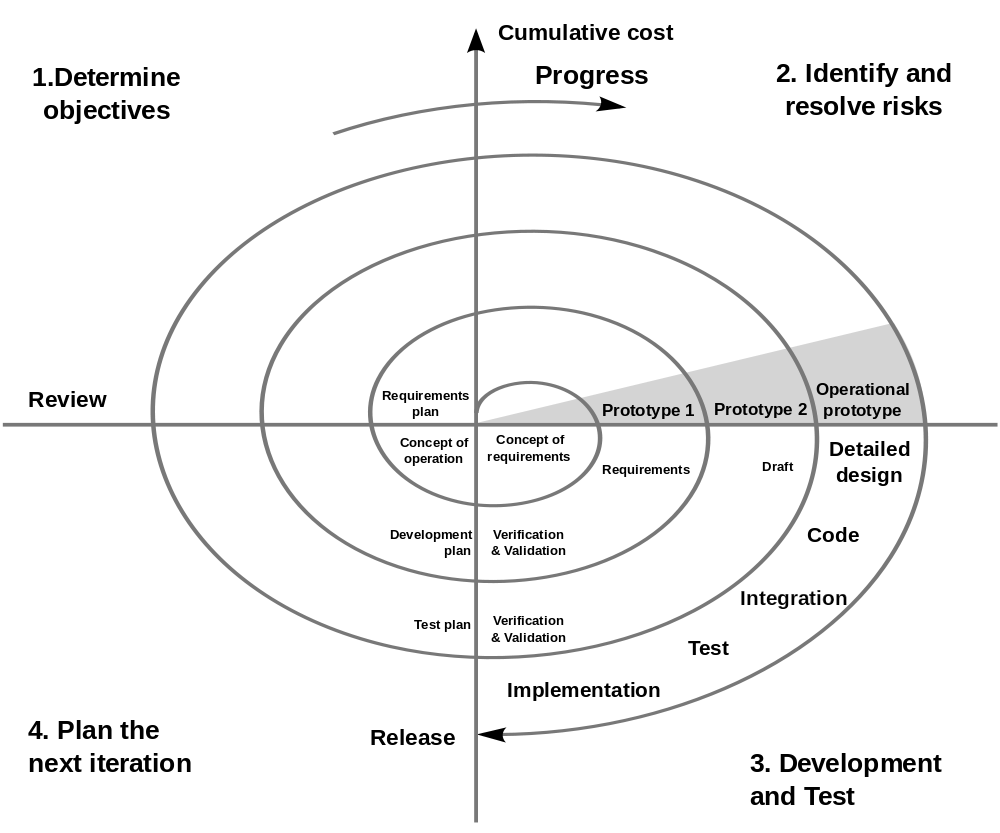
\includegraphics[width=0.75\textwidth]{imag/IMG17.png}
				\caption{Representación del desarrollo en espiral.} 
	\label{fig:Desarrollo en espiral.}	
	\end{center}
\end{figure}


\section{Plan de trabajo}
\hspace{1cm} Para conseguir los objetivos expuestos anteriormente se ha seguido una planificación dividida en estas fases:

\begin{itemize}
	\item \textbf{Formación en Python y C++:} Necesaria para entender el código existente de los antecedentes
directos de este Trabajo Fin de
Grado en los que me he basado y para crear el mío propio. Con el conocimiento y seguimiento de tutoriales y ejercicios básicos de c/c++ y una serie de guías de ayuda fue el  primer paso de aprendizaje.
	\item \textbf{Formación con herramientas:} Introducción a JdeRobot para comprender el funcionamiento de la infraestructura y saber todas las herramientas con las que se contaba. Para ello se realizaron una serie de programas simples en los cuales trabajabas con distintos robots y con diferentes herramientas, teniendo así los primeros contactos con programación de robots simulados y reales. Familiarización con el simulador Gazebo, el simulador utilizado preferentemente en JdeRobot, en el hubo que crear el entorno de simulación sobre el cual se basaría el programa de vuelo del drone. Formación con la herramienta VisualStates de programación con autómatas.	
	\item \textbf{Aprendizaje e integración del componente de autolocalización:} Necesario para conocer el funcionamiento y el uso del componente Slam-VisualMarkers, y manejar los parámetros y las balizas con las que trabaja, conseguir con él una correcta autolocalización del drone y tambien obtener los errores de la herramienta y extraerlos de los errores de pilotaje.
	\item \textbf{Aprendizaje e integración del control de aterrizaje:} Para adaptarlo a la aplicación dentro de un autómata finito de estados y a su vez crear un propio sistema de despegue del drone.
	\item \textbf{Dinseño y desarrollo del algoritmo para el pilotaje:} Se han explorado dos algoritmos, por un lado seguimiento de puntos separados y por otro lado el de seguimiento de trayectorias continuas. Ambos capaces de gobernar el movimiento del drone para seguir las rutas en 3D.
	\item \textbf{Integración de todos los módulos de navegación en un autómata de estados finito desarrollado con VisualStates:} El programa se ha desarrollado sobre la aplicación Visual States, la cual he tenido que aprender para conseguir introducir todas las etapas y que funcionase correctamente. 
	\item \textbf{Validación experimental:} Para comprobar y validar el correcto funcionamiento de las fases anteriores tanto unitariamente como del sistema global se realizaron una serie de experimentos en entornos simulados. Con estas pruebas se detectaron posibles comportamiento erróneos que corrigiéndolos se consiguió estabilidad en el sistema acercándonos a su viabilidad en entornos reales.   
\end{itemize}
